% Chapter 1: Introduction to LLMs: Beyond the Hype
\chapter{Introduction to LLMs: Beyond the Hype}

Large Language Models (LLMs) have rapidly moved from research labs to practical applications, capturing the imagination of 
technologists and the public alike. For software engineers, LLMs represent a new class of powerful tools and components that can be
 integrated into systems to solve complex problems, automate tasks, and create novel user experiences. This chapter aims to demystify
  LLMs, providing a foundational understanding geared specifically towards software engineering perspectives and applications.

\section{What are LLMs? A Software Engineer's Perspective}

At its core, a Large Language Model is an advanced type of artificial intelligence algorithm specifically designed to understand, 
generate, and manipulate human language on a large scale. These models are trained on vast quantities of text data, enabling them to 
produce coherent and contextually relevant responses to a wide array of prompts. It's crucial for software engineers to view LLMs not 
as sentient entities possessing genuine understanding, but as sophisticated pattern-matching and generation engines. Their ability to 
recognize, summarize, translate, predict, and generate content makes them powerful components within larger software systems.

The utility of LLMs extends beyond just human language. They can be applied to other "languages" or scenarios where communication of 
different types is needed, such as understanding protein and molecular sequences in biology or, more directly relevant to software engineers, 
generating and understanding software code.

A fundamental characteristic that engineers must grasp is that LLMs operate on principles of probability, not on a basis of truth or 
genuine comprehension. They predict "what word should come next" to produce fluent text, but they do not inherently understand the reality 
of what they describe. This probabilistic nature means their outputs are generations based on learned patterns. This makes them highly 
effective for tasks like code generation or text summarization, which benefit from strong pattern recognition and fluent output. However, 
it also implies that their outputs may require external verification or grounding, especially when factual accuracy is critical. 
This understanding is paramount for designing robust software systems that leverage LLMs, as it necessitates incorporating mechanisms 
for validation, error handling, and potentially human oversight in critical applications.

\section{Core Concepts: Input, Output, and Tokens}

Interacting with an LLM involves several core concepts that software engineers need to understand to effectively harness their capabilities.

\subsection*{Input ("Prompt")}
The process begins when a user or a system provides text input to the LLM. This input is commonly referred to as a "prompt". 
The prompt serves as the instruction or the context based on which the LLM will generate a response. For software engineers, 
crafting effective prompts---a practice known as prompt engineering---is a key skill for guiding the LLM to produce desired outputs.

\subsection*{Output ("Generation")}
Based on the input prompt and the patterns it has learned during training, the LLM generates an output, typically in the form of text. 
This output is often called a "generation." The quality and relevance of the generation depend heavily on the prompt, the model's training, 
and various configurable parameters.

\subsection*{Tokens}
LLMs don't process text as whole words or characters directly. Instead, they break down text into smaller units called "tokens". 
A token can be a word, a part of a word (sub-word), or even a single character, depending on the specific tokenization scheme used by the model. 
For software engineers, understanding tokens is important because API costs for many commercial LLMs are based on the number of tokens processed (both input and output). 
Additionally, LLMs have maximum token limits for their input context and output generation, which can influence how applications are designed.

\subsection*{Parameters (Model Weights)}
LLMs possess millions, or even billions, of "parameters". These parameters are essentially the weights and biases within the model's neural 
network that are learned during the training process. They collectively define the model's behavior and its ability to understand language patterns 
and generate human-like text. Generally, a higher number of parameters correlates with greater model capability but also demands more computational 
resources for training and inference.

\subsection*{Temperature}
This is a crucial parameter that engineers can control when generating text with an LLM. Temperature influences the randomness of the LLM's output. 
A lower temperature (e.g., 0.0 to 0.3) makes the output more deterministic and focused; the LLM will tend to pick the most probable next token. 
This is useful for tasks requiring factual accuracy or predictable outputs, like code generation or direct question answering. 
A higher temperature (e.g., 0.7 to 1.0 or higher) results in more random, creative, and diverse outputs, as the LLM is more likely to choose less probable tokens. 
This can be beneficial for creative writing or brainstorming but may also increase the likelihood of generating nonsensical or irrelevant responses. 
Finding the right temperature setting is often a matter of experimentation based on the specific application needs.

Grasping these concepts allows software engineers to move beyond treating LLMs as black boxes. Tokenization, parameter counts, and especially temperature 
are practical levers for controlling LLM behavior, managing API costs, and optimizing the performance and predictability of LLM-integrated applications.

\section{A Glimpse Inside: Simplified LLM Internals}

While a deep dive into the mathematical intricacies of LLMs is beyond the scope of this book, a simplified understanding of their internal workings is 
beneficial for software engineers. LLMs learn from immense volumes of text data through a process often involving unsupervised learning. 
During this phase, the model is not given explicit instructions on what to do with the data but rather learns to identify patterns, structures, and 
relationships between words and concepts embedded within the text.

The fundamental mechanism by which most LLMs operate is "next token prediction". Given a sequence of input tokens, the model calculates the probability 
distribution for all possible next tokens in its vocabulary and then selects one (or samples from the distribution) to continue the sequence. T
his process is repeated, with each newly generated token being added to the input sequence for predicting the subsequent token, allowing the LLM to 
generate coherent and contextually relevant text autoregressively.

The development of an LLM typically involves two main stages:

\begin{itemize}
    \item \textbf{Pre-training:} This is where the model learns general language understanding from a massive, diverse corpus of text data 
    (e.g., books, articles, websites). The goal is to build a foundational understanding of language, grammar, common knowledge, and reasoning abilities.
    \item \textbf{Fine-tuning:} After pre-training, a model can be further trained on a smaller, more specific dataset to adapt its capabilities 
    to a particular task or domain. For example, a general pre-trained model can be fine-tuned on a dataset of medical research papers to specialize 
    in medical language, or on a corpus of code to improve its code generation abilities. Fine-tuning can also adjust the model's tone, style, or factual knowledge.
\end{itemize}

The seemingly intelligent outputs of LLMs, such as their ability to generate working code, refactor existing code , or engage in complex dialogue, 
all stem from this core probabilistic "next token prediction" mechanism. This understanding is vital for engineers when debugging unexpected model 
outputs or so-called "hallucinations." Hallucinations, where an LLM generates incorrect or fabricated information despite sounding plausible , 
are not entirely random errors. They can be seen as logical outcomes of the probabilistic generation process when the input prompt is ambiguous, 
poorly constrained, or leads the model into areas of the learned pattern-space that were sparsely represented in its training data. 
Recognizing this helps in developing better prompt engineering strategies and in designing systems that can validate or provide corrective 
feedback for LLM outputs, especially in critical applications.

\section{LLMs and Data: The Role of GPUs in Processing}

The computational demands of training and running Large Language Models are substantial, and Graphics Processing Units (GPUs) play a critical 
role in handling these intensive workloads. LLM computations, particularly during the training and inference (generation) phases, are heavily 
dominated by matrix-matrix multiplication operations. GPUs, with their massively parallel architecture, are exceptionally well-suited for 
performing these types of calculations far more efficiently than traditional CPUs.

A key factor in LLM performance on GPUs, especially during inference, is memory bandwidth. While computational power (measured in FLOPS - 
Floating Point Operations Per Second) is important, the speed at which data (model parameters, intermediate calculations) can be moved between 
the GPU's main memory (VRAM) and its compute units often becomes the bottleneck, particularly for the decoding phase of text generation. 
This means that simply having a GPU with high FLOPS might not guarantee the best performance if its memory bandwidth is insufficient for the 
model's size and the desired batching strategy.

LLM text generation typically involves a two-step process on GPUs :

\begin{itemize}
    \item \textbf{Prefill (Prompt Processing):} When a prompt is first given to the LLM, the tokens in this input prompt are processed in parallel 
    by the GPU. This phase is generally compute-bound.
    \item \textbf{Decoding (Token Generation):} After the initial prompt processing, text is generated one token at a time in an 
    autoregressive manner. Each newly generated token is appended to the input sequence and fed back into the model to produce the next token. 
    This phase is often memory-bandwidth-bound.
\end{itemize}

To optimize these processes, several techniques are employed:

\begin{itemize}
    \item \textbf{KV Caching (Key-Value Caching):} During the autoregressive decoding phase, the attention mechanism (discussed in the next section) 
    needs to consider all previously generated tokens. Without optimization, this would involve significant re-computation. 
    KV caching addresses this by saving the intermediate "key" and "value" states from the attention layers for previously processed tokens. 
    These cached values are then reused in subsequent token generation steps, avoiding redundant calculations and significantly speeding up the decoding process.
     Effective management of the KV cache memory is crucial for good inference performance.
    \item \textbf{Quantization:} This technique involves reducing the numerical precision of the model's parameters (weights). 
    For example, parameters might be converted from 32-bit floating-point (FP32) or 16-bit floating-point (FP16) to 8-bit integers (INT8) or even 
    4-bit integers (INT4). Smaller data types mean the model takes up less VRAM and, critically, less data needs to be moved between memory and compute units, 
    which can speed up inference, especially in memory-bandwidth-bound scenarios. However, quantization can sometimes lead to a slight degradation in model accuracy,
     so a balance must be struck.
\end{itemize}

For software engineers involved in deploying or managing LLM applications, understanding these GPU processing characteristics is vital. 
It informs choices about hardware selection, model optimization strategies (like quantization), batching techniques for requests, and 
overall system architecture to achieve desired performance targets (like Time To First Token (TTFT) and Time Per Output Token (TPOT) ) 
and manage operational costs effectively.

\section{Understanding Transformers: The Engine of LLMs}

The vast majority of modern Large Language Models, including well-known ones like GPT, LLaMa, and Claude, are built upon a neural network 
architecture called the Transformer. Introduced in a 2017 paper titled "Attention is All You Need" , the Transformer architecture revolutionized
 natural language processing by providing a more effective way to handle sequential data, like text, compared to previous architectures such as 
 Recurrent Neural Networks (RNNs) and Long Short-Term Memory (LSTMs) networks.

For software engineers, having a conceptual understanding of the Transformer's key components is beneficial for appreciating why LLMs are so 
powerful and how they fundamentally operate, without needing to delve into the deepest mathematical details.

\subsection*{Key Components of the Transformer Architecture}

\begin{itemize}
    \item \textbf{Input Embeddings and Tokenization:} As discussed earlier, input text is first broken down into tokens. Each token is then converted 
    into a numerical vector called an "embedding". These embeddings represent the tokens in a high-dimensional space where tokens with similar meanings 
    or contexts are located closer to each other. This numerical representation is what the model actually processes.
    \item \textbf{Positional Encoding:} Unlike RNNs that process tokens sequentially, Transformers can process all tokens in an input sequence in 
    parallel. This parallelism is a key to their efficiency but means the model doesn't inherently know the order of the tokens. Positional encoding 
    solves this by adding information to each token's embedding that indicates its position within the sequence. This allows the model to understand 
    and utilize word order, which is crucial for language comprehension.
    \item \textbf{Self-Attention Mechanism:} This is arguably the most critical innovation of the Transformer. The self-attention mechanism allows the 
    model, when processing a particular token, to look at all other tokens in the input sequence and weigh their importance or relevance to the current token.
    In essence, each token calculates an "attention score" with every other token in the sequence. These scores determine how much "focus" or "attention" to pay
     to other tokens when generating a representation for itself. This allows the model to capture long-range dependencies and contextual relationships between words, 
     no matter how far apart they are in the sequence. For example, in the sentence "The cat didn't chase the mouse, because it was not hungry," self-attention 
     helps the model understand that "it" refers to "cat".
    \item \textbf{Multi-Head Attention:} Instead of performing self-attention just once, Transformers use "multi-head" attention. This means the self-attention 
    mechanism is run multiple times in parallel, with each "head" learning different types of relationships or focusing on different aspects of the input sequence. 
    The outputs from these multiple heads are then combined, allowing the model to capture a richer and more diverse set of contextual information.
    \item \textbf{Feed-Forward Networks (FFN):} After the attention mechanism has processed the tokens and incorporated contextual information, each token's 
    representation is passed through a position-wise Feed-Forward Network. This FFN consists of a few fully connected layers and is applied independently to each token. 
    Its role is to further process and transform each token's representation, adding more non-linearity and complexity to the model's understanding.
    The formula is generally FFN(x)=max(0,xW$_{1}$+b$_{1}$)W$_{2}$+b$_{2}$.
    \item \textbf{Encoder-Decoder Architecture (High-Level):} The original Transformer model was designed for machine translation and featured an encoder-decoder 
    structure.
    \begin{itemize}
        \item The Encoder processes the input sequence (e.g., a sentence in English) and builds a rich contextual representation of it. Encoder-only models 
        are good for tasks requiring input understanding, like classification.
        \item The Decoder takes the encoder's output (and potentially other inputs) and generates the output sequence (e.g., the translated sentence in French). 
        Decoder-only models are good for generative tasks like text completion. Many modern LLMs primarily used for text generation (like GPT models) are 
        decoder-only architectures, while others used for tasks like summarization might use the full encoder-decoder structure or be encoder-only (like BERT).
    \end{itemize}
    \item \textbf{Stacking Layers:} Transformer models are typically "deep," meaning they consist of multiple encoder blocks (in the encoder) 
    and multiple decoder blocks (in the decoder) stacked on top of each other. Each block contains the self-attention and feed-forward network components. 
    This stacking allows the model to learn increasingly complex and abstract representations of the input data as it passes through the layers.
\end{itemize}

\subsection*{Conceptual Block Diagram of a Transformer Block}
A simplified textual representation of a single Transformer block (which could be an Encoder block or a Decoder block, with slight variations) would look like this:

\begin{figure}[h!]
\centering
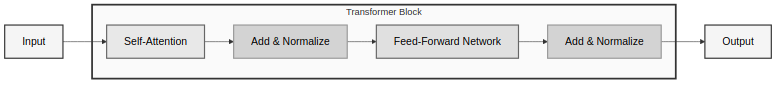
\includegraphics[width=\textwidth]{diagrams/transformer_block.png}
\caption{Conceptual Block Diagram of a Transformer Block}
\label{fig:transformer_block}
\end{figure}

\textbf{Explanation of Diagram:}
\begin{itemize}
    \item \textbf{Input:} The process starts with token embeddings that have positional encoding added to them.
    \item \textbf{Multi-Head Self-Attention:} This input goes into the multi-head self-attention mechanism, where tokens interact and weigh each other's importance.
    \item \textbf{Add \& Norm Layer:} The output of the attention layer is typically added to the original input to that layer (a residual connection) 
    and then normalized (Layer Normalization). This helps with training stability and information flow.
    \item \textbf{Feed-Forward Network:} The normalized output then passes through a position-wise feed-forward network for further transformation.
    \item \textbf{Add \& Norm Layer:} Another residual connection and layer normalization are applied.
    \item \textbf{Output:} The output of this block can then be fed into the next identical block (if stacking multiple blocks) or, if it's the final block, 
    to a final output layer that converts the processed representations into token probabilities for generation. Decoder blocks would also have an additional 
    multi-head attention layer that attends to the output of the encoder (in encoder-decoder architectures).
\end{itemize}

The self-attention mechanism is the pivotal innovation that enables Transformers to effectively handle long-range dependencies in text, a significant 
improvement over prior architectures like RNNs and LSTMs which struggled with this due to their sequential nature and issues like vanishing gradients. 
For software engineers, this superior ability to maintain context over much longer inputs is critical for tasks such as understanding entire code files, 
lengthy technical documents, or extended conversations, making LLMs far more versatile and powerful. 